\section{Methodology}
\label{chap:methodology}
In the methodology I aim to coherently outline the methods used in the study, including datasets, models, generation techniques, metrics and more. I will start off with an overview of the datasets used, followed by an explanation of the pre-processing steps that were performed to prepare the data for our model. Afterwards, I will outline the generation pipeline, from training the model to generating lyrics, and then I will go over the experimental setup and the evaluative framework, including sections expanding upon all of the metrics used, as well as our objectives for the parameter tuning process. Lastly, I will go over training and architecture of our model, followed by an extensive overview of the various decoding algorithms employed for generation.

\subsection{Datasets}
\label{sec:datasets}

As previously mentioned, I have selected and retrieved two datasets for study, one for each of the language models. The two chosen datasets have been picked on the basis of their high quality content, their size and their accessibility.

\subsubsection{Rap Lyrics Dataset}
\label{rap-dataset}

The rap lyrics (RP) dataset chosen for our lyrics-based model was pulled from the large dataset database \textit{Kaggle} and is titled \textit{Hip-Hop Encounters Data Science}. The dataset consists of lyrics from 37 rap artists split up into individual text files, which in total consists of $\sim$186k lines, $\sim$1.42m words and $\sim$7.84m characters. The average word length is $\sim$5.17 characters and the average line consists of $\sim$5.52 words. The vocabulary size of the dataset is 38.7k words. Each of the text files was loaded in sequentially and saved in a single array, from which they were processed.

\subsubsection{General Purpose Dataset}
\label{general-dataset}

The general dataset chosen for the general-purpose (GP) language model is \textit{WikiText-2} \cite{WikiText2016} downloaded from the website \textit{PapersWithCode}\footnote{\url{www.paperswithcode.com/dataset/wikitext-2}}. It is made up of \textit{good} and \textit{featured} articles from scraped from Wikipedia, condensed into 3 text files: (\textit{training}, \textit{test} and \textit{validation}), all retaining original punctuation and numbers. Here, good articles are chosen via an nomination and assessment system, and are therefore widely considered high-quality articles, making up just $\sim1/177$ of all articles\footnote{\url{https://en.wikipedia.org/wiki/Wikipedia:Good_articles}}. Featured articles articles are similar, but are instead chosen directly by Wikipedia editors, on the criteria of being amongst "the best articles Wikipedia has to offer"\footnote{\url{https://en.wikipedia.org/wiki/Wikipedia:Featured_articles}}.

As to mimic the size of our rap lyrics dataset, I will only be using the training data from WikiText2. After from very light extraction pre-processing, the dataset consists of $\sim$1.98m words $\sim$10.86m characters. The average word length is $5.43$ characters and the size of the dataset vocabulary is $\sim$ 78.6k words. The entire dataset was loaded in and saved in a single string, from which they were then pre-processed further.

\subsection{Pre-processing}
\label{sec:pre-processing}

Before moving on to the creation of our models, we first have to prepare the data for being fed to our models. This involves both properly loading in the data, converting it to the desired format, here characters, and subsequently removing all unwated characters, punctuation, etc. While similar types of pre-processing is required for both datasets, as to properly standardize the data as to not accidentally bias the training / generation, there are differences, which we will discuss momentarily. Consequently, we will examine the process of readying the datasets independently, begining with our RL dataset.

\subsubsection{RL Dataset Processing}
\label{rap-pre-processing}

To prepare the lyrics data for being fed into our model, we first performed a number of pre-processing steps, in order to make it more suitable. Firstly, the text data had to be cleaned up through removal of redundant empty lines and fixing other minor anomalies in the data, such as converting the data to all lowercase and removing lines that were shorter than 8 characters. This was done to remove both empty- and 1-word lines, which might otherwise have a negative impact on the model during training, due to the degree to which they differ from regular lyrics / text. It would also serve to make the next step of processing have a larger impact on the shape of the data, the step in question being the introduction of \textless{}endLine\textgreater{} and \textless{}endVerse\textgreater{} tokens. These would function in much the way as their names might suggest, the \textless{}endLine\textgreater{} tokens being added to the end of each line and the \textless{}endVerse\textgreater{} tokens being added to the end of each verse (signalled by upcoming empty lines which, in our dataset, always denoted the end of a verse).

This also allowed the data to more easily be represented as a single continuous string and, chiefly, to potentially capture the nature of end-rhymes, and the structure of rap lyrics more generally. This approach was inspired by Potash et al. (2015) \cite{potash-etal-2015-ghostwriter}, in which they employed this strategy to great effect within their word-based model. Another reason for this approach was that it would hopefully amplify the effectiveness of the \textit{memory cells} in our Long Short-Term Memory model, attempting to draw upon the network's ability to “remember” configurations of word/characters from previous sequences. A very simplistic example of what I would ideally like to “teach” the model is the relation between a line ending with the tokens “m, o, n, e, y, \textless{}endLine\textgreater{}” and the next line “h, o, n, e, y, \textless{}endLine\textgreater{}.

It should be noted that, in theory, this approach seems more likely to be successful at generating correct / common rhymes in the case of word-level tokens. This is due to the underlying difference between pronunciation for characters in different contexts, which is both more common and severe than varying pronunciations found amongst identical words. However, its employment in a character-based model might allow for rhymes that are more “original” to occur, as the generated results are not previously seen words, but rather character tokens which combine to make words. If successful, this might help to emulate the rhyming technique of “imperfect”- or “half” rhymes, employed by many rappers, an oft-cited example being “Eminem” and his recurring fondness of rhyming “orange” with “door-hinge” or “syringe”, twisting word pronunciations to force unusual rhymes.

All together, these preliminary processing steps decreased the number of characters in our dataset by $\sim$43k, from $\sim$7.484m to $\sim$7.441m $\approx0.575\%$ reduction. 

The second section of pre-processing consisted of two processing steps:
\begin{itemize}
    \item Replacing non-ascii character e.g. non-English characters (foreign alphabets like Hiragama or Cyrillic), accented characters (á), BOM characters (\textbackslash{}ufeff) etc.
    \item Removing unwanted punctuation, which in our case is the following list: \\ "\#\$\%\slash\&\(\)\*+/\textless{}\textgreater{}=@[]\^\_`\{\|\}$\sim$\textbackslash{}”
\end{itemize}

Both of these pre-processing steps, while important, were fairly subtle in their reduction of the dataset. The removal of all non-ascii characters reduced the dataset by 9.840 characters, $\approx0.132\%$ reduction, and removal of the unwanted punctuation by 22.433 characters, $\approx0.303\%$ reduction, leaving us with $\sim$7.408 million characters, $\approx0.44\%$ reduction.

\subsubsection{GP Dataset Processing}
\label{general-pre-processing}

The majority of the pre-processing steps performed on the general-purpose dataset mirrored those performed on the lyrics dataset. Initially, the redundant empty lines were removed, the data was converted to all lowercase and lines shorter than 8 characters were removed. The \textless{}endVerse\textgreater{} and \textless{}endLine\textgreater{} tokens were also added as before, this time with slightly altered purposes. The \textless{}endLine\textgreater{} token remained much the same, in that it was used to denote the end of lines. The \textless{}endVerse\textgreater{} token was this time used to better denote the boundaries between different sections/headings, and was therefore inserted in between the end of a section and the headline of the forthcoming section.

This allowed our model to gather an understanding of where new sections start and previous sections end, without having to use characters which already has purpose\footnote{Prior to pre-processing, the new sections in the dataset were formatted as: "= = = NEW SECTION = = =", which used up a lot of space while also employing already existing purposeful tokens (=).}, while simultaneously doing so with just a single character. Overall, this whole process actually increased the size of the datase from $\sim$10.84m characters to $\sim$10.86, an increase of $19.528\approx0.18\%$ of the total dataset.

Then, as with the lyrics dataset, non-ascii characters were removed, as well as unwanted punctuation, further reducing the size of the dataset by $14.149$ characters $\approx0.13\%$ (for the characters) and $104.345$ characters $\approx0.971\%$ (for the punctuation). There was also a number of other minor dataset-specific pre-processing steps performed, such as removal of spaces before commas and removal of spaces around hyphens, the combination of all of which resulted in a reduction of $241.406$ characters, $\approx2.3\%$.

Lastly, the size of the dataset was altered to better fit the size of our rap lyrics dataset, reducing it from $\sim$10.5m characters to $\sim$7.41m characters, making the sizes of the datasets functionally identical ($\sim$99,97\%). This was simply done by slicing the excess $\sim$3.1m characters off the end of the dataset.

\subsection{Generation Pipeline}
\label{sec:generation-pipeline}

My approach to the generation of lyrics consists of using a Long Short-Term Memory model based on character tokens, teaching the model to predict and eventually generate lyrics on the basis of our dataset. During training, a version of the model is saved every training epoch, if the current epoch was superior to the previous iteration, which in our case was defined as having a lower loss value, specifically \textit{categorical cross-entropy}. The reason behind saving a separate model at every incremental improvement, was to compare the performance gained versus number of training epochs, and also examine potential over-fitting issues that our model might run into.
After the training of the model(s) concluded, I initiated testing with 5 different generation/decoding techniques, as to identify which was best suited for generating novel, coherent and interesting lyrics. This process consisted of continuous testing of decoding parameters, as we will see shortly. Once this initial tuning had been completed, and the optimal parameters decided on, we were ready to test the lyrics generation capabilities of our model.

% TABLE OF EXAMPLES OF RHYME DENSITIES FOR VARIOUS ARTIST FROM THE DATASET

\begin{table*}[htb!]
    \begin{center}
    \caption{Examples of rhyme densities for various artists from our dataset}
    \vspace{6pt}
    \label{tab:rdtable}
    \bgroup
    \def\arraystretch{1.3}
    \begin{tabular}{c|l|c}
        \textbf{Rank} & \multicolumn{1}{c|}{\textbf{Artist}} & \textbf{Rhyme Density} \\[0.1cm]\hline
        1. & Earl Sweatshirt & 1.217 \\
        2. & Montana of 300 & 1.210 \\
        3. & Joey Badass & 1.167 \\
        4. & ASAP Rocky & 1.158 \\
        5. & Action Bronson & 1.151 \\\hdashline
        10. & Logic & 1.123 \\\hdashline
        16. & Nas & 1.097 \\
        17. & Eminem & 1.093 \\\hdashline
        19. & The Notorious B.I.G  & 1.066 \\
        20. & Tupac & 1.066 \\\hdashline
        32. & Kendrick Lamar & 1.019 \\
        33. & Childish Gambino & 1.001 \\
        34. & Tyler The Creator & 0.998 \\
        35. & Immortal Technique & 0.998 \\
        36. & Ice Cube & 0.924 \\
        37. & Andre 3000 & 0.883 \\
        \hline
    \end{tabular}
    \egroup
    \end{center}
\end{table*}

\subsection{Setup and Evaluation}
\label{sec:setup+eval}

The approach to evaluating the output of text-generation models is undoubtedly one of most disputed areas in computational creativity. This is in part due to the issue of evaluation criteria fluctuating from paper to paper, making it very difficult to make conclusive comparisons between the output of different models, even in the case of similar model objectives. On top of that, in this setup, we will be dealing with a number of different generative techniques, all with their own parameters, not the mention the required tuning of our language model itself. Therefore, the evaluation process will be split up into multiple parts: fine-tuning of our language model, selection of optimal intra-method parameters for the various generative techniques and, lastly, overall inter-method evaluation of the fine-tuned generation techniques. While extensive manual evaluation of generated lyrics is not within the scope of this paper, we will be looking at a number of textual features throughout, related to the objective at hand. The final evaluation of our model will performed by examining the model’s ability to generate rhymes, write coherent test, and make use of a large vocabulary, as a means of generating novel lyrics. For more information on evaluating generated text, see sections \cref{sec:extending-evaluation} and \cref{sec:eval-of-generated-text}, as well as the accompanying sources.

To start off with, let us take a look at the different evaluation metrics we will be using throughout, to evaluate the specific task we are trying to optimize for.

\subsubsection{Rhyme Density}
\label{sec:rhyme-density}

One of the most common and valuable components for both automatically generated rap lyrics \cite{potash-etal-2015-ghostwriter}, \cite{Malmi_2016}, \cite{PotashPeter2016ECLG} and poetry \cite{goncalo-oliveira-2017-survey}, \cite{GoncaloOliveiraHugo2014PGwP} is \textit{rhymes}. There are different ways to evaluate rhymes in texts, depending on what metric you are trying to gauge, one of the more promising ones being the recently proposed \textit{rhyme density} (RD). This metric was first introduced by Malmi et al. (2016) \cite{Malmi_2016} and, quickly summarized, represents the average multisyllabic assonance rhyme lengths per word.  To compute the rhyme density, I have used the implementation by Eric Malmi, as was used in the original paper, and is available on github\footnote{\url{https://github.com/ekQ/raplysaattori}}.

In \cref{tab:rdtable} we see that the artist with the best rhyme density, according to the songs included in our dataset, is \textit{Earl Sweatshirt} with a rhyme density of 1.217. At the bottom of the table, we find \textit{Andre 3000} with a rhyme density of ust 0.883. Looking at our entire dataset, as can be seen in \cref{tab:complete-rd-table}, the average rhyme density is $\sim$1.074.

\subsubsection{Initial Evaluation Metrics}
\label{sec:initial-eval-metrics}

\paragraph{Average Unique Words/verse (AUW):\\[6pt]}
\label{para:avg-unique-words/v}

The first metric we employ is average unique words/verse, defined as the average number of unique words per generated verse, which exists in the vocabulary\footnote{The vocabulary against which the generated text is tested is made up of all the words from the datasets combined with the ViewVC dictionary. More information can be found regarding the dictionary at \url{https://svnweb.freebsd.org/*docroot*/help_dirview.html}}. This is a very simple baseline metric, which manages to accomplish two things: one, it wheats out sets of parameters that result in complete nonsense, as words that do not exist in our vocabulary are not counted. And two: it penalises repeating the same word over and over again in the same verse, as this is only counted as a single word, in the context of comparing it to the training vocabulary.

\paragraph{Duplicate Lines/verse (DL):\\[6pt]}
\label{para:dupes/v}

The second metric for our initial evaluation is the number of repeated lines within a verse. This acts in conjunction with the first metric to combat the persistent issue of repetition in text produced by language models, as shown by Holtzmann et al. \cite{HoltzmanAri2019TCCo}. This metric is even more coarse than the previous one, as it only considers any given line a repetition if it matches the previous line \textit{exactly}. Nevertheless, it does add the ability to distinguish between parameter settings which are similar in their number of unique real words per verse, if one contains more duplicate lines.

\paragraph{Total Vocabulary Size (VS):\\[6pt]}
\label{para:total-vocab-size}

The third and last of the initial metrics, measures the total vocabulary size, allowing us a fuller perspective of how interesting the text produced might be, as well as how coherent. As with the previously mentioned metrics, they become substantially more powerful when evaluated in conjunction, as each individually has flaws and shortcomings, which might become less detrimental by inclusion of metrics without those specific issues.

\subsubsection{Other Evaluation Metrics}
\label{sec:other-eval-metrics}

\paragraph{Average Line Length (ALL):\\[6pt]}
\label{sec:avg-sent-length}

Average Line Length is, much as the name suggests, defined as the average line length over all lines in a configuration’s training. This metric will be employed after the initial rough sort has commenced, as it will be less valuable when used to measure incoherent text, most of which we hope to have filtered out after the preliminary tuning. It works to evaluate the similarity between the structure of the generated text, to that of real rap lyrics.

\paragraph{Average Word Length:\\[6pt]}
\label{para:avg-word-length}

Average Word Length follows the same principals as ALL and is also not employed prior to finishing the preliminary evaluations for the exact same reason(s). It assists in evaluating the complexity of the generated text and can, in conjunction with other metrics such as \hyperref[para:avg-unique-words/v]{AUW}, help measure the novelty of the generated text.

\paragraph{Average Number of Duplicate Bigrams (ANDB):\\[6pt]}
\label{para:avg-dupe-bigrams}

The last evaluation metric we employ is ANDB, which is a measure to count bigram duplicates within the same verses. There is certainly an argument to be made for including this metric in our preliminary parameter exploration, but one of the reasons for not including it, is that we have already included the more coarse DL metric, which would seem to better fit the task at hand, i.e. sorting out just the \textit{worst} configurations. The main reason, however, is the uncertainty regarding whether this metric accurately represents \textit{bad rap}. While we expect this to be the case, the consequences of being wrong might entail eliminating one or more promising parameter configurations, and is therefore naturally something we hope to avoid at (almost) all costs.

\paragraph{Total Number of Non-words (TNNW):\\[6pt]}
\label{total-non-words}

The metric works by counting the number of words in a given text which does not appear in the specified vocabulary, which helps in gauging the legibility of the generated text. This works well in conjunction with other quality metrics, to define a acceptable limit above which the generated text might be considered "suitable".

These 7 fairly simple metrics, as well as the more advanced metric \hyperref[sec:rhyme-density]{\textit{RD}}, will in conjunction with manual human evaluation, help to guide our choices of configurations, and illuminate which decoding techniques and configurations are performing the best.

% \subsubsection{Preliminary Tuning Objectives}
% \label{sec:prelim-tuning-objects}

% After evaluating the parameters according to the initial evaluation metrics, we hope to be left with a sparser range of parameters which are more effective than their peers in generating natural sounding, non-repetitive language. Due to this goal, initial tests are more limited, both with regards to sample size and comprehensiveness, than the ones coming after. They are merely in place to avoid having to slavishly evaluate hundreds of different parameter configurations, many of which will be generating wholly unsuitable outputs. This will subsequently allow us more time to do more comprehensive fine-grained evaluation of the best performing initial parameters.

\subsection{LSTM Model}
\label{sec:lstm-model}
The type of model chosen for both of our text generation tasks is, as previously mentioned, a Recurrent Neural Network (RNN) with Long Short-Term Memory (LSTM). The LSTM is unique due to its \textit{memory cell}, which consists of an input gate, output gate, forget gate and cell/cell memory, which enables its “memory”. More explicitly, each of these cells have their own bias vectors and computation of the hidden layer at each stage is a complex nonlinear combination of gate, cell, and hidden vectors \cite{Malmi_2016}. The reason behind choosing this model in particular, is its proven ability to embed long-distance dependencies, by the inherent merit of its architectural design. The specific implementation of the LSTM model was done using Keras with TensorFlow 2. LSTM were also preferable over other models as they are proven model architectures when it comes to modelling language, irrespective of whether the language in question is C++ code \cite{karpathy_2015} or rap lyrics \cite{potash-etal-2015-ghostwriter}, \cite{PotashPeter2016ECLG}, due to their previously mentioned ability to map long-range dependencies. Furthermore, within the limited scope of automatic generation of rap lyrics, the LSTM model have recently been the preferred choice, making it the obvious choice for further exploration.

Another very promising architecture is the encoder transformer model, which has recently emerged as one of the fastest and most impressive models for an assortment of NLP tasks. For more information of transformers, see \cref{chap:discussion} and Vaswani et al. (2017) \cite{VaswaniAshish2017AIAY}.

\subsubsection{Architecture}
\label{sec:model-architecture}

The architecture of our models consists of 5 layers, 2x2 LSTM layers with 512 neurons, followed by a dropout layer with $dropout=0.2$. The final layer is a fully connected dense layer with 49 neurons, representing the 49 different characters in our vocabulary. The input LSTM layer takes 80 inputs, each being a character represented as a one-hot Boolean vector of length equal to our vocabulary.

\subsubsection{Training}
\label{sec:model-training}

For training the lyrics model, I experimented with a number of different parameters, batch sizes $\{b=32, \ldots, 2^{n+4} \mid n \in{1,\ldots,6}\}$ different input segment sizes $\{40,60,80\}$ different initial learning rates as well as various types of model architecture parameters such as dropout rates and layer sizes. I settled on what seemed to produce the best results in terms of minimizing loss, training the model with batch sizes of 128 for a total of 232 epochs of 19.293 steps, after which model improvement became rare and negligible. After each epoch, the model was saved if it succeeded in minimizing the loss function, namely categorical cross-entropy. The model was trained using the Adam optimization algorithm \cite{KingmaDiederikP2014AAMf} and initialized with a learning rate of $1.0^{-3}$. Subsequently, the learning rate would update automatically if it had seen no improvement in loss for 3 consecutive epochs. The final model terminated with a loss value of 1.3267 and was trained with a learning rate of $lr=1.0^{-12}$. After the model had reached the aforementioned loss value, it was trained for 8 additional epochs with two reductions of the learning rate, eventually reaching $lr=1.0^{-14}$, after which the model was stopped, as no improvement had been found, and it was assumed that the model had come close to reaching a local minimum.

The same approach was mirrored for the training of the general-purpose model, which started plateauing around epoch 204 with a current learning rate of $lr=1.0^{-11}$ and a categorical cross entropy loss of 1.3924. While loss value was noticeably higher than for our RL model, it should still suffice for the given testing purposes, serving as a useful baseline against which to test the ability of the lyrics-model to emulate rap.

\subsection{Generation Techniques and Decoding Algorithms}
\label{sec:generation-techs}

As mentioned previously, there are a number of different generations techniques/decoding algorithms used with language models, generation quality varying greatly between them. In researching generative techniques, I tested a number of different generative techniques, both to see which approach would suit the LR model the best, but also exploratorily to gauge the shortcomings and capabilities of different approaches. On top of the decoding framework, there are also other strategies one can employ in tandem with some of the decoding strategies, one of the which is “temperature sampling”.

Generally, there are two overarching types of generation techniques: \textit{deterministic}- and \textit{stochastic} decoding, \hyperref[sec:det-simple]{some} techniques falling somewhere in-between by merit of their ability to be used in conjunction with other methods. Deterministic decoding is defined as selecting the highest probability token from the available candidates. As opposed to selecting the token with the highest probability, stochastic decoding techniques "randomly" select the next token on the basis of its conditional probability distribution.

In the following section I will start off by outlining the various algorithms, the inspirations behind them, how they work, and what their benefits and shortcomings are, in a text-generation framework.

\subsubsection{Deterministic Decoding: Simple Greedy Search}
\label{sec:det-simple}
Greedy decoding is, as the name suggests, an algorithm which falls under the header “greedy algorithms” meaning that it follows the problem-solving heuristic of making the locally optimal choice at each time-step, without taking upcoming steps into account. In other words, this algorithm is a novice chess player who does not plan ahead for optimal long-term game states, but just attempts to make the move that improves the immediate game-state most successfully. In the context of decoding, the greedy approach simply returns the maximum value in the probability distribution over the vocabulary.

One of the most apparent flaws for greedy approach in NLG is its tendency to get stuck in loops, due to the nature of always picking the highest probability token. An example of this, produced by our own model using greedy decoding, can be seen in \cref{fig:greedyrepeat}.

% FIGURE 1 - EXAMPLE OF GENERATIVE REPETITION USING GREEDY ENCODING
\begin{figure}[H]
\centering
\captionsetup{width=1\linewidth, position=bottom}
{\setlength{\fboxsep}{10pt}
    \fbox{%
        \begin{minipage}{10em}
            \textit{he won’t follow us \\
            yeah yeah, yeah, yeah \\
            yeah, yeah, yeah, yeah, \\
            yeah, yeah, yeah, yeah}
        \end{minipage}
    }
\captionof{figure}{Example of generative repetition using Greedy Encoding}
\label{fig:greedyrepeat}}
\end{figure}

Here the generated text starts out as we would expect, but very quickly degenerates into a loop, only repeating the same word \textit{yeah} over and over again. Also, this issue is not limited to just repeating the same word, as seen here, and might also manifest itself as a loop of continuously repeating phrases.

\subsubsection{Deterministic Decoding: Beam Search}
\label{sec:det-beam}

Beam search is a more advanced decoding algorithm than simple greedy search, in that it does not only return the highest probability from the distribution, but considers the probability of all states, expanding a predetermined number $\beta$ of the best states, at each time step. The naming convention is based off of the shape that the explored and expanded nodes form, if you graph the search, and the value of the parameter might be thought of as the width of the “beam”, as illustrated in \cref{fig:beamsearch}

% BEAM SEARCH FIGURE
\begin{figure*}[ht!]
    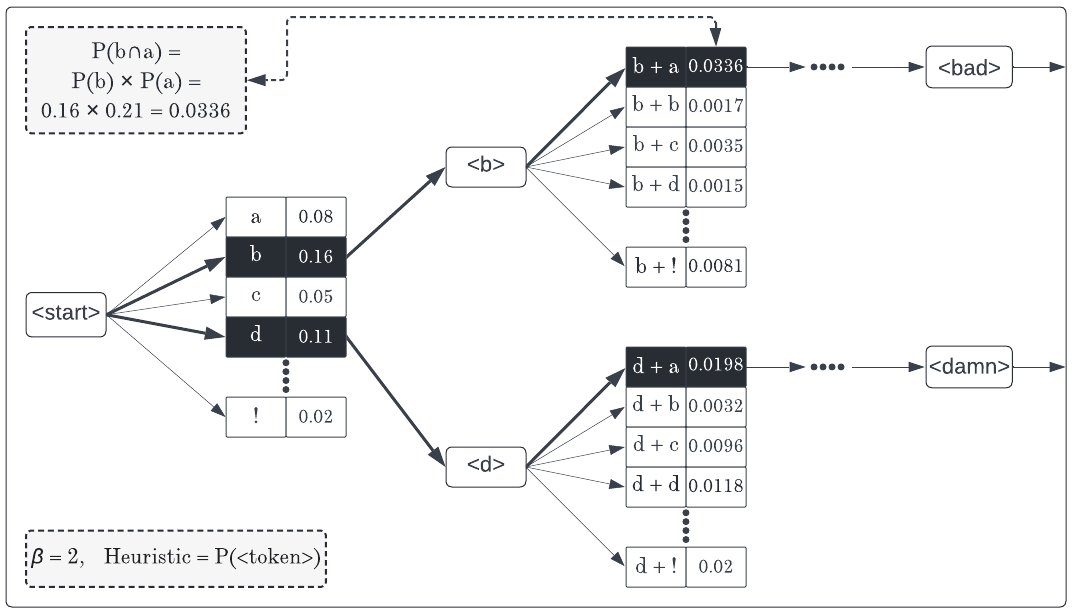
\includegraphics[width=\textwidth, keepaspectratio=true]{figures/Beam Search (Character-based LM) (1).png}
    \caption{Beam Search Example}
    \label{fig:beamsearch}
\end{figure*}

To build upon the chess analogy from before, beam search represents a more experienced player who maps out future game states for $\beta$ number of “best moves”. In this analogy, the depth is equal to how many moves the player looks ahead, paying attention only to the $\beta$ most promising moves at each time-step. This has the obvious advantage over simple greedy search, in that while grabbing the free \textbf{pawn} might seem like the best option \textit{right now}, you might be missing a move capturing a free \textbf{queen} a few steps down the road.

How this functions in practice in our LM is by multiplying the cumulative probability of the previously explored node with each of the individual probabilities of the currently explored node, adding them to a list a potential “candidate nodes”. When all the current nodes have been explored, equal to $\beta \cdot V \mid \beta = beam\;width$ (number of promising nodes to keep), $V = vocabulary\;size$, only the $\beta$ best nodes are retained, which will then be explored next.

Though certainly better than greedy search, beam search also falls prey to some of the same pitfalls as greedy search. While the beam width allows it to explore a greater number of promising options, it does not stop it from entering a looping state, producing the same type repeating of sequences as we saw with beam search in \cref{fig:greedyrepeat}, as it \textit{still} picks the best option it is presented with. One of the proposed ways of remedying this issue is using what is called \textit{n-gram penalties} \cite{PaulusRomain2017ADRM} \cite{Klein2017OpenNMT}. While this does manage to avoid repetition, it also presents issues for both character- and word-based LMs: Character-based models face the issues of difficulties in spelling at low n-gram values and also being unable to use previously used content words for higher n-gram values. This latter issue also pertains to word-based models at $n = 1$ or $n = 2$, and as higher values are introduced, the benefit of avoiding repetition stars to wane, making the solution less useful.

Lastly, as mentioned, despite its benefits over simply greedy search, beam search is still a greedy decoding algorithm at its core, only selected the highest probabilities according to its beam-width, meaning that it will never consider values outside of it’s hard cut-off. One of the ways to deal with this hard cut-off point, which is at the centre of all deterministic decoding algorithms, is to use randomness, specifically \textit{sampling}.

\subsubsection{Stochastic Decoding: Temperature Sampling}
\label{sec:sto-temp}

The first sampling/stochastic decoding method is actually one rarely used as a standalone decoding strategy in practice, as it is rather used in conjunction with the other stochastic decoding strategies such like \textit{top-k} and \textit{nucleus} sampling.

Temperature sampling was originally inspired by statistical thermodynamics, where high temperatures means that low energy states are more likely to be encountered. In practice, it is a function whose objective it is to impose varying degrees of randomness into the generation process by dividing the ”logits” by the a “temperature” and then applying the SoftMax function, from which we can sample our probabilities. In other words, sampling from a temperature of 0 is equal to doing a simple greedy search while higher temperatures impose more randomness and can, at the extremes ($\geq$1), start breaking down the structure completely, the ideal temperature lying somewhere in-between.

\subsubsection{Stochastic Decoding: Top-K Sampling}
\label{sec:sto-top-k}

Top-k sampling was originally proposed by Fan et al. (2018) \cite{FanAngela2018HNSG} as decoding technique for hierarchical story generation. Top-k sampling is a simple yet effective decoding scheme in which at every time step, the \textit{top-k} probabilities are retrieved, redistributed using SoftMax and then a value is chosen “randomly”, that is, based on its conditional probability. This has the advantage over regular temperature scaling, in its ability to remove the tail, meaning that the ability to remove the vast majority of low-probability tokens, only concerning itself with the $k$ number of best options. This is especially useful in word-based language models, as in they have tails, i.e. vocabularies, many orders of magnitude larger than those of character-models.\footnote{This is due how next-token prediction language models work. The models draw from a vocabulary of tokens, picking the according to its decoding algorithm, e.g. the most likely for greedy decoding algorithms. The difference lies in that, for character-based models, the vocabulary is equal to the dictionary of characters the model has seen in the training set, usually consisting of $\sim$50 tokens, depending on whether or not punctuation is included. In the case of word-based models, the tokens in the vocabulary is equal to all the \textit{words} the model has seen in the training data, meaning that instead of a vocabulary size of 50 tokens, you have one of 50.000+ tokens, as is the case with GPT-3 \cite{BrownTomB2020LMaF}, making the "tail", i.e. the number of unlikely tokens, much longer.}

One of the pitfalls of using \textit{top-k} sampling, is that it does not dynamically adapt the number of included probabilities, the \textit{k}, meaning that its behaviour varies a lot between \textit{narrow} and \textit{broad} distributions, resulting in difficulties in the selection of a one-size-fits-all value for \textit{k}. This is especially problematic for character-based models, as the distributions from which it samples is very small. This further increase the carefulness with which values of \textit{k} have to be chosen, as even the smallest increments to \textit{k}, +1, are sizable on the scale of the vocabulary. In our case, $k + 1$ would result in the additional inclusions of $\sim$2\% of our \textit{entire} vocabulary.

\subsubsection{Stochastic Decoding: Nucleus Sampling}
\label{sec:sto-top-p}

\textit{Nucleus} sampling, also known as \textit{top-p} sampling, was first proposed by Holtzman et al. (2019) \cite{HoltzmanAri2019TCCo} as an alternative to \textit{top-k} sampling, and in many ways, it succeeded. The two techniques are almost identical, the only difference being that the choice of \textit{k} in nucleus sampling is relative to the distribution of the probabilities, adding some much needed dynamicity. It does this by selecting \textit{k} on the basis of the cumulative probabilities \textit{n} being at least equal top \textit{p} portion of the probability mass. In other words, \textit{p} denotes the percentage of the probability mass to be included in our sampling, i.e., the \textit{nucleus}. This avoids is avoiding the issue that top-k sampling faces in finding a value for \textit{k} which is suitable for both narrow and broad distributions, making the varying vocabulary sizes less of an issue.